\chapter{Architettura Logica}
\section{Cosa è l'Architettura Logica?}
\begin{minipage}{0.5\textwidth}
    \begin{figure}[H]
        \centering
        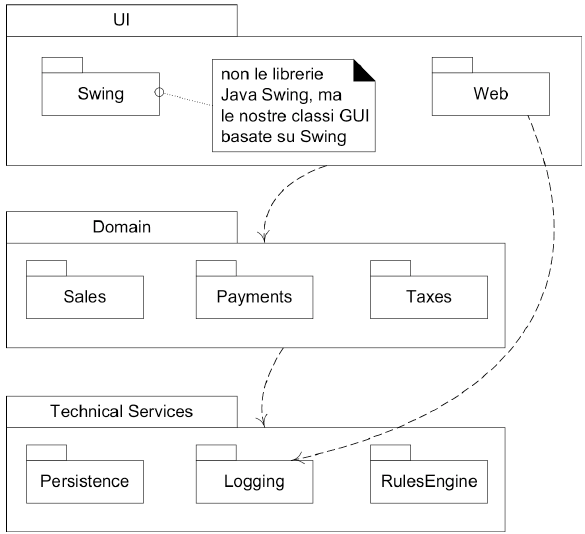
\includegraphics[scale=0.65]{Immagini/Schermata_20260712_110437.png}
    \end{figure}
\end{minipage}
\hfil
\begin{minipage}{0.35\textwidth}
    \begin{itemize}
        \item L'architettura logica di un sistema software è l'organizzazione su larga scala delle classi software in package, sottoinsiemi e strati \\
        \item Uno stile comune per l'architettura logica è l'architettura a strati
    \end{itemize}
\end{minipage}

\section{Architettura a Strati}
\subsection{Cosa è uno stato?}
\begin{itemize}
    \item Uno strato è un gruppo a grana molto grossa di classi, package, o sottosistemi, che ha della responsabilità coese a un aspetto importante il sistema
    \begin{itemize}
        \item Gli strati più alti ricorrono ai servizi degli strati più bassi (normalmente non avviene il contrario)
    \end{itemize}
    \item Gli starti di un'applicazione software comprendono normalmente:
    \begin{itemize}
        \item Presentazione - Interfaccia utente
        \item Logica applicativa o strato del dominio - elementi che rappresentano concetti del dominio
        \item Servizi tecnici
    \end{itemize}
\end{itemize}
\subsection{Architettura a strati stretta}
Uno strato può solo richiamare i servizi dello strato immediatamente sottostante
\subsection{Architettura a strati rilassata}
Uno strato più alto può richiamare i servizi di strati più bassi di diversi livelli

\section{Cosa è un architettura software?}
Un architettura software è:
\begin{itemize}
    \item L'insieme delle decisioni significative sull'organizzazione di un sistema software
    \item La scelta degli elementi strutturali da cui è composto il sistema e delle relative intefacce
    \item Insieme al loro comportamento specificato dalla collaborazione tra questi elementi
    \item La composizione di questi elementi strutturali e comportamentali in sottosistemi via via più ampi
    \item È lo stile architetturale che guida questa organizzazione
\end{itemize}

\chapter{Diagramma dei Package}
\section{A cosa serve?}
\begin{itemize}
    \item L'architettura logica può essere illustrata mediante un diagramma dei package 
    \begin{itemize}
        \item Uno strato può essere modellato come un package UML
    \end{itemize}
    \item Un package UML può ragruppare qualunque cosa (classi, altri package, casi d'uso, \dots)
    \begin{itemize}
        \item È molto comune l'annidamento di package
        \item Per mostrare la dipendenza tra i package viene utilizzata una dipendenza UML
        \item Un package UML rappresenta un namespace cossichè è possibile definire due classi con lo stesso nome su package diversi
    \end{itemize}
\end{itemize}

\section{Definizioni: Livelli, Strati e Partizioni}
\begin{itemize}
    \item \textbf{Livello :} Solitamente indica un nodo fisico di elaborazione
    \item \textbf{Strato :} Una sezione verticale dell'architettura
    \item \textbf{Partizione :} Una divisione orizzontale di sottosistema di uno strato 
\end{itemize}
\begin{figure}[H]
    \centering
    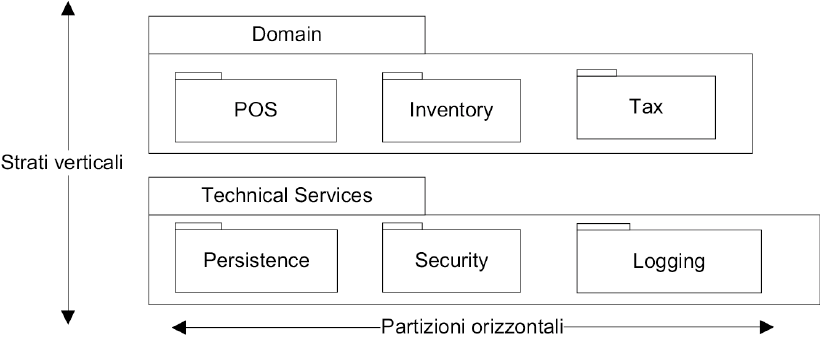
\includegraphics[scale=0.8]{Immagini/Schermata_20260712_120930.png}
\end{figure}

\newpage
\section{Progettazione degli strati}
\subsection{Gerarchia degli stati}
\begin{itemize}
    \item Organizza la struttura logica di un sistema in strati separati con responsabilità distinte e correlate, con una separazione netta e coesa degli interessi
    \begin{itemize}
        \item Gli strati inferiori servizi generali e di basso livello
        \item Gli strati superiori sono più specifici per l'applicazione
    \end{itemize}
    \item Collaborazioni e accoppiamenti vanno dagli strati più alti a quelli più bassi
    \item L'obiettivo è la suddivisione di un sistema in un insieme di elementi software che, per quanto possibile, possano essere sviluppati e modificati ciascuno indipendentemente dagli altri
\end{itemize}
\subsection{Scelta comune per gli strati}
\subsubsection{UI}
\begin{minipage}{0.5\textwidth}
    \begin{figure}[H]
        \centering
        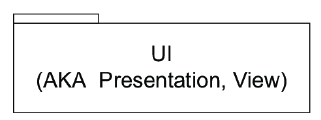
\includegraphics{Immagini/Schermata_20260712_113614.png}
    \end{figure}
\end{minipage}
\hfil
\begin{minipage}{0.35\textwidth}
    \begin{itemize}
        \item Finestre della GUI
        \item Report
        \item Interfaccia vocale
    \end{itemize}
\end{minipage}

\subsubsection{Application}
\begin{minipage}{0.5\textwidth}
    \begin{figure}[H]
        \centering
        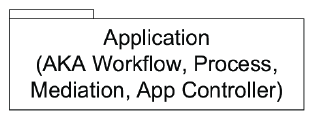
\includegraphics{Immagini/Schermata_20260712_113747.png}
    \end{figure}
\end{minipage}
\hfil
\begin{minipage}{0.35\textwidth}
    \begin{itemize}
        \item Gestisce richieste dello strato UI
        \item Workflow
        \item Stato delle sessioni
        \item Transizioni tra finestre/pagine
        \item Consolidamente/trasformazione di dati disparati per la presentazione
    \end{itemize}
\end{minipage}

\subsubsection{Domain}
\begin{minipage}{0.5\textwidth}
    \begin{figure}[H]
        \centering
        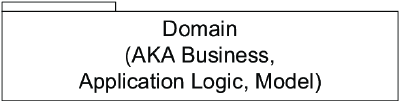
\includegraphics[scale=0.8]{Immagini/Schermata_20260712_113925.png}
    \end{figure}
\end{minipage}
\hfil
\begin{minipage}{0.35\textwidth}
    \begin{itemize}
        \item Gestisce richieste dello strato Application
        \item Implementazione delle regole di dominio 
        \item Servizi di dominio
        \begin{itemize}
            \item I servizi possono essere utilizzati da una sola applicazione, ma sono possibili anche servizi di interesse per più applicazione
        \end{itemize}
    \end{itemize}
\end{minipage}

\subsubsection{Business Infrastructure}
\begin{minipage}{0.5\textwidth}
    \begin{figure}[H]
        \centering
        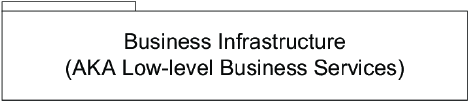
\includegraphics[scale=0.8]{Immagini/Schermata_20260712_114156.png}
    \end{figure}
\end{minipage}
\hfil
\begin{minipage}{0.35\textwidth}
    \begin{itemize}
        \item Servizi aziendali molto generali e di basso livello util
    \end{itemize}
\end{minipage}

\subsubsection{Technical Service}
\begin{minipage}{0.5\textwidth}
    \begin{figure}[H]
        \centering
        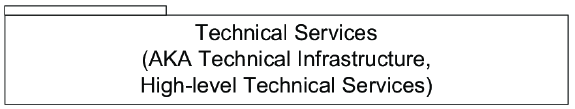
\includegraphics[scale=0.7]{Immagini/Schermata_20260712_120657.png}
    \end{figure}
\end{minipage}
\hfil
\begin{minipage}{0.35\textwidth}
    \begin{itemize}
        \item Servizi tecnici e framework di livello alto
    \end{itemize}
\end{minipage}

\subsubsection{Foundation}
\begin{minipage}{0.5\textwidth}
    \begin{figure}[H]
        \centering
        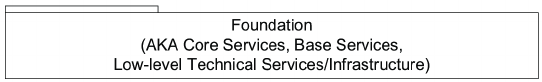
\includegraphics[scale=0.7]{Immagini/Schermata_20260712_121217.png}
    \end{figure}
\end{minipage}
\hfil
\begin{minipage}{0.35\textwidth}
    \begin{itemize}
        \item Servizi tecnici e framework di livello basso livello, strutture di dati, thread, matematica
    \end{itemize}
\end{minipage}

\subsection{Principio di separazione Modello-Vista}
\begin{itemize}
    \item Gli oggetti di dominio (modello) non devono essere connessi o accoppiati direttamente agli oggetti UI
    \begin{itemize}
        \item Non permettere a un oggetto di dominio Sale di avere un riferimento a un oggetto finestra JFrame di Java Swing
    \end{itemize}
    \item Non mettere la logica applicativa nei metodi di un oggetto è l'interfaccia utente
    \begin{itemize}
        \item Gli oggetti UI dovrebbero solo inizializzare gli elementi dell'interfaccia utente, ricevere eventi UI, e delegare le richieste di logica applicativa agli oggetti non UI
    \end{itemize}
\end{itemize}